\documentclass[10pt,a4paper,british]{article}
\usepackage[utf8]{inputenc}
\usepackage{fullpage}
\usepackage{graphicx}
\usepackage{fancyhdr}
\usepackage{comment}
\usepackage{occi}
\setlength{\headheight}{13pt}
\pagestyle{fancy}

% default sans-serif
\renewcommand{\familydefault}{\sfdefault}

% no lines for headers and footers
\renewcommand{\headrulewidth}{0pt}
\renewcommand{\footrulewidth}{0pt}

% header
\fancyhf{}
\lhead{GWD-R}
\rhead{\today}

% footer
\lfoot{occi-wg@ogf.org}
\rfoot{\thepage}

% paragraphs need some space...
\setlength{\parindent}{0pt}
\setlength{\parskip}{1ex plus 0.5ex minus 0.2ex}

% some space between header and text...
\headsep 13pt

\setcounter{secnumdepth}{4}

\begin{document}

% header on first page is different
\thispagestyle{empty}

GWD-R \hfill  Thijs Metsch, Platform Computing\\
OCCI-WG \hfill  Andy Edmonds, Intel\\
\rightline {Ralf Nyrén, Aurenav}\\
\rightline {October 14, 2010}\\
\rightline {Updated: \today}

\vspace*{0.5in}

\begin{Large}
\textbf{Open Cloud Computing Interface - Core}
\end{Large}

\vspace*{0.5in}

\underline{Status of this Document}

This document provides information to the community regarding the
specification of the Open Cloud Computing Interface. Distribution is
unlimited.


\underline{Obsoletes}

This document obsoletes GFD-xxx [REFERENCE].

\underline{Copyright Notice}

Copyright \copyright Open Grid Forum (2009-2010). All Rights Reserved.

\underline{Trademarks}

OCCI is a trademark of the Open Grid Forum.

\underline{Abstract}

This document, part of a document series, produced by the OCCI working
group within the Open Grid Forum (OGF), provides a high-level
definition of a Protocol and API. The document is based upon
previously gathered requirements and focuses on the scope of important
capabilities required to support modern service offerings.


\newpage
\tableofcontents
\newpage

\section{Introduction}
The Open Cloud Computing Interface (OCCI) is a RESTful Protocol and
API for all kinds of Management tasks. OCCI was originally initiated
to create a remote management API for IaaS%
\footnote{Infrastructure as a Service}
model based Services, allowing for the development of interoperable tools for
common tasks including deployment, autonomic scaling and monitoring.
%
It has since evolved into an flexible API with a strong focus on
interoperability while still offering a high degree of extensibility. The
current release of the Open Cloud Computing Interface is suitable to serve many
other models in addition to IaaS, including e.g.~PaaS and SaaS.

In order to be modular and extensible the current OCCI specification is
released as a suite of complimentary documents which together form the complete
specification.
%
The documents are divided into three categories consisting of the OCCI Core,
the OCCI Renderings and the OCCI Extensions.
%
\begin{itemize}
\item The OCCI Core specification consist of a single document defining the
 OCCI model. The OCCI model is the core of OCCI and can be manipulated by {\em
 renderings} and expanded through {\em extensions}.
\item The OCCI Rendering specifications consist of multiple documents each
 describing a particular rendering of the OCCI model. Multiple renderings can
 manipulate the same instance of the OCCI model and will automatically support
 any additions to the model which follow the extension rules defined in OCCI
 Core.
\item The OCCI Extension specifications consist of multiple documents each
 describing a particular extension of the OCCI model. The extension documents
 describe additions to the OCCI model defined within the OCCI specifiction
 suite.
\end{itemize}
%
The current specification consist of three documents, one in each catogery.
Future releases of OCCI may include additional rendering and extension
specifications. The documents of the current OCCI specification suite are:

\begin{description}
\item[OCCI Core] describes the formal definition of the the OCCI model
\cite{occi:core}.
\item[OCCI HTTP Rendering] defines how to manipulate the OCCI model using the
RESTful OCCI API \cite{occi:http}. The document defines how the OCCI model can
be communicated and thus serialized using the HTTP protocol.
\item[OCCI Infrastructure] contains the definition of the OCCI Infrastructure
extension for the IaaS domain \cite{occi:infrastructure}. The document defines
additional resource types, their attributes and the actions that can be taken
on each resource type.
\end{description}


\section{Notational Conventions}
All these parts and the information within are mandatory for
implementors (unless otherwise specified). The key words "MUST", "MUST
NOT", "REQUIRED", "SHALL", "SHALL NOT", "SHOULD", "SHOULD NOT",
"RECOMMENDED", "MAY", and "OPTIONAL" in this document are to be
interpreted as described in RFC 2119 \cite{rfc2119}.

\textbf{Andy: we need to state that this document as part of the current document set,
supersedes all previous documents.}


\section{OCCI Core}
The Open Cloud Computing Interface is a boundary protocol and API
that acts as a service front-end to a provider's internal management
framework. Figure~\ref{fig:placement} shows OCCI's place in a
provider's architecture.
\begin{figure}[h]
	\centering
	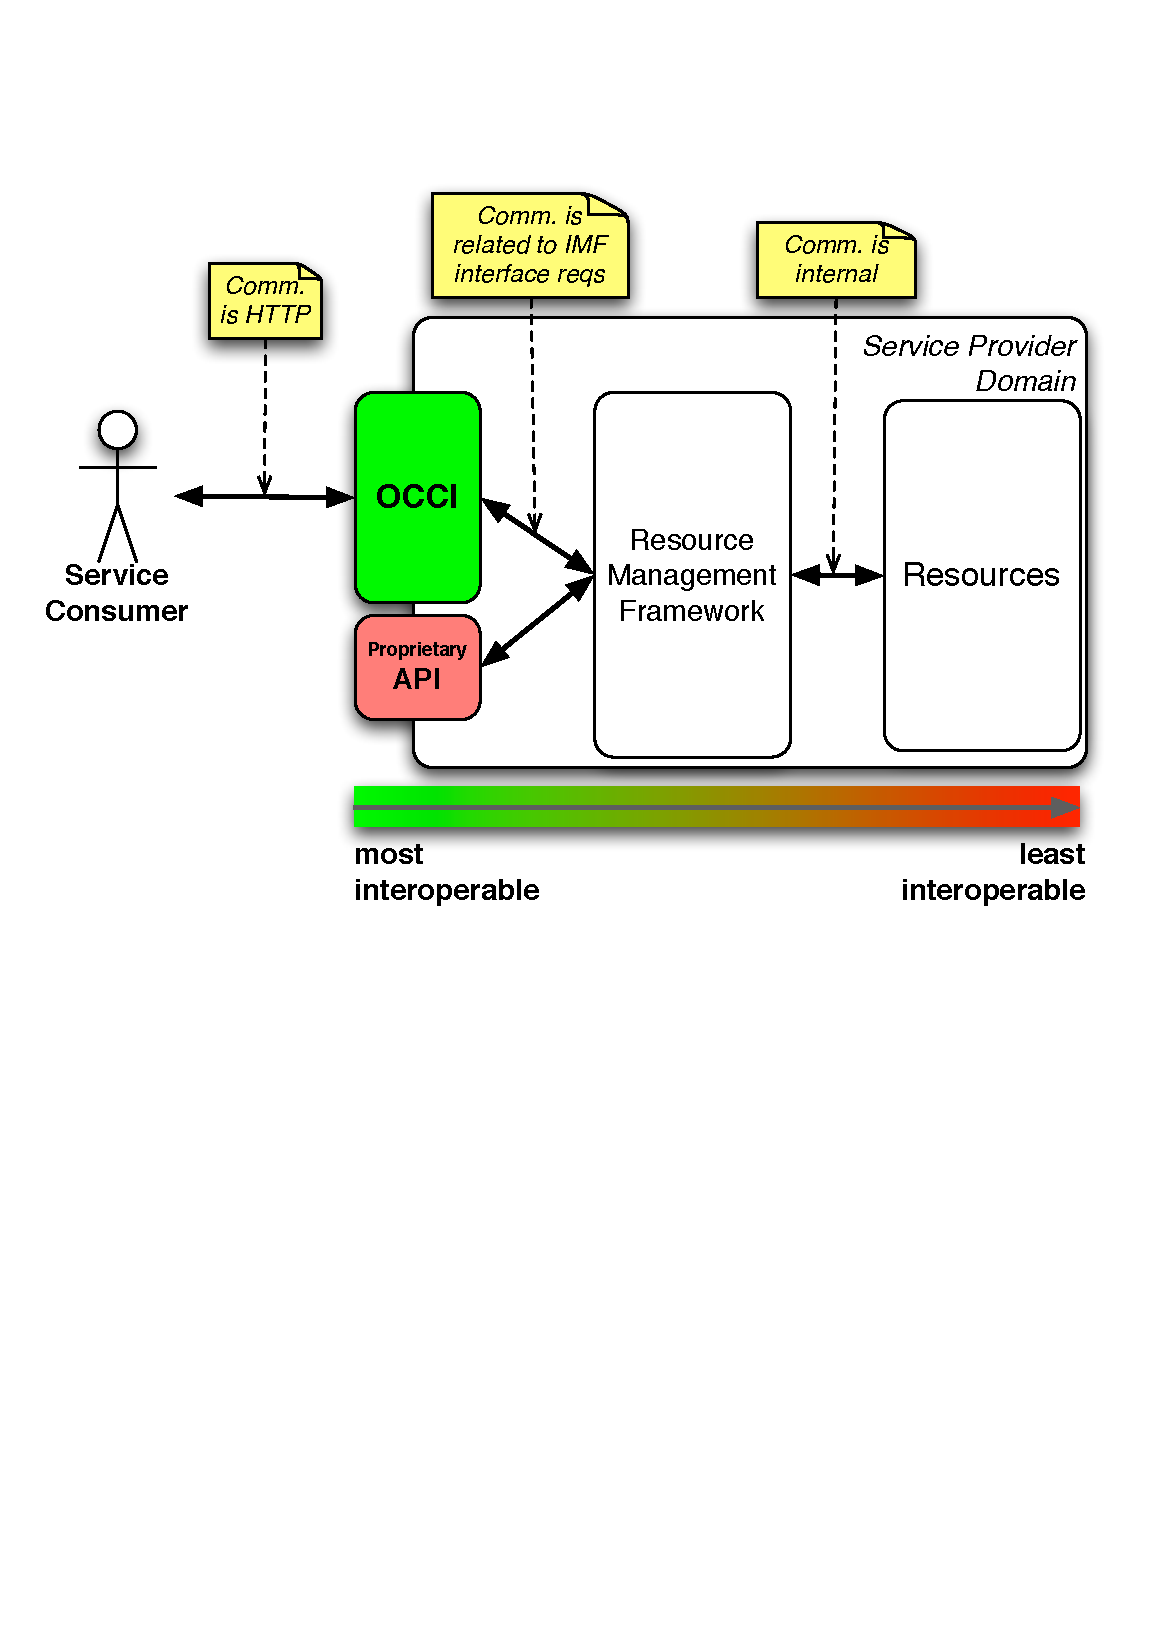
\includegraphics[scale=0.5]{figs/occi-intro.pdf}
	\caption{OCCI's place in a provider's architecture}
	\label{fig:placement}
\end{figure}
Service consumers can be both end-users and other system instances, OCCI is
suitable for both cases. The key feature is that OCCI can be used as a
management API for all kinds of resources while at the same time maintaining a
high level of interoperability.

This document, the OCCI Core specification, define the OCCI model. The OCCI
model is the core of the specification suite and the model can be manipulated by
renderings and expanded through extensions. In itself, the model is only useful
for a very limited set of use cases. However, it provides the basis for
renderings and extensions to build upon.

\section{OCCI model}
The OCCI model defines a representation of instance types which can be
manipulated through an OCCI Rendering implementation. It is not a
``meta-model'' \cite{meta-model-ref-something}. It is merely a first level
abstraction of real world resources, including the means to identify, classify,
associate and extend those resources. 

A fundamental feature of the OCCI model is that it can be extended in such a
way that any extension will be discoverable and visible to an OCCI client at
run-time. An OCCI client can connect to an OCCI implementation with
domain-specific extensions, without knowing anything in advance, and still be
able to provide a decent end-user experience. For example, a web-based OCCI
client could easily be reused as the management tool for a wide variety of
services.

The OCCI model can be extended through a regular inheritance model but also
using a ``mix-in'' like model. The mix-in model only applies at the instance
level, i.e.~the ``object level'', and thereby differs from the more common uses
of the mix-in concept. A mix-in in OCCI can never be applied to a type, only to
an instance.

\subsection{Overview}

The heart of the OCCI model is the \hl{Resource} type. Any resource exposed
through OCCI is a \hl{Resource} or a sub-type thereof.
A resource can be e.g.~a virtual machine, a job in a job submission system, a
user, etc.
%
The \hl{Resource} type contains a number of common attributes that
domain-specific \hl{Resource} types inherit. The \hl{Resource} type is
complemented by the \hl{Link} type which associates one \hl{Resource} instance
with another.
%
The \hl{Link} type also contains a number of common attributes that
domain-specific \hl{Link} types inherit.

\hl{Entity} is an abstract type which both \hl{Resource} and \hl{Link} inherit.
Each sub-type of \hl{Entity} is identified by a unique \hl{Kind} instance.
%
The \hl{Kind} type is the core of the classification and identification
system built into the OCCI model. \hl{Kind} is a specialisation of
\hl{Category} and introduces additional capabilities in terms of \hl{Action}s.

The last type defined by the OCCI model is the \hl{Mixin} type. An instance of
\hl{Mixin} can be associated with a resource instance, i.e.~a sub-type of
\hl{Entity}, to ``mix-in'' additional capabilities at run-time.
%
For compliance with OCCI Core, all of the types defined in the OCCI model MUST
be implemented.

\begin{figure}[!h]
{\centering \resizebox*{0.9\columnwidth}{!}{\rotatebox{270}
      {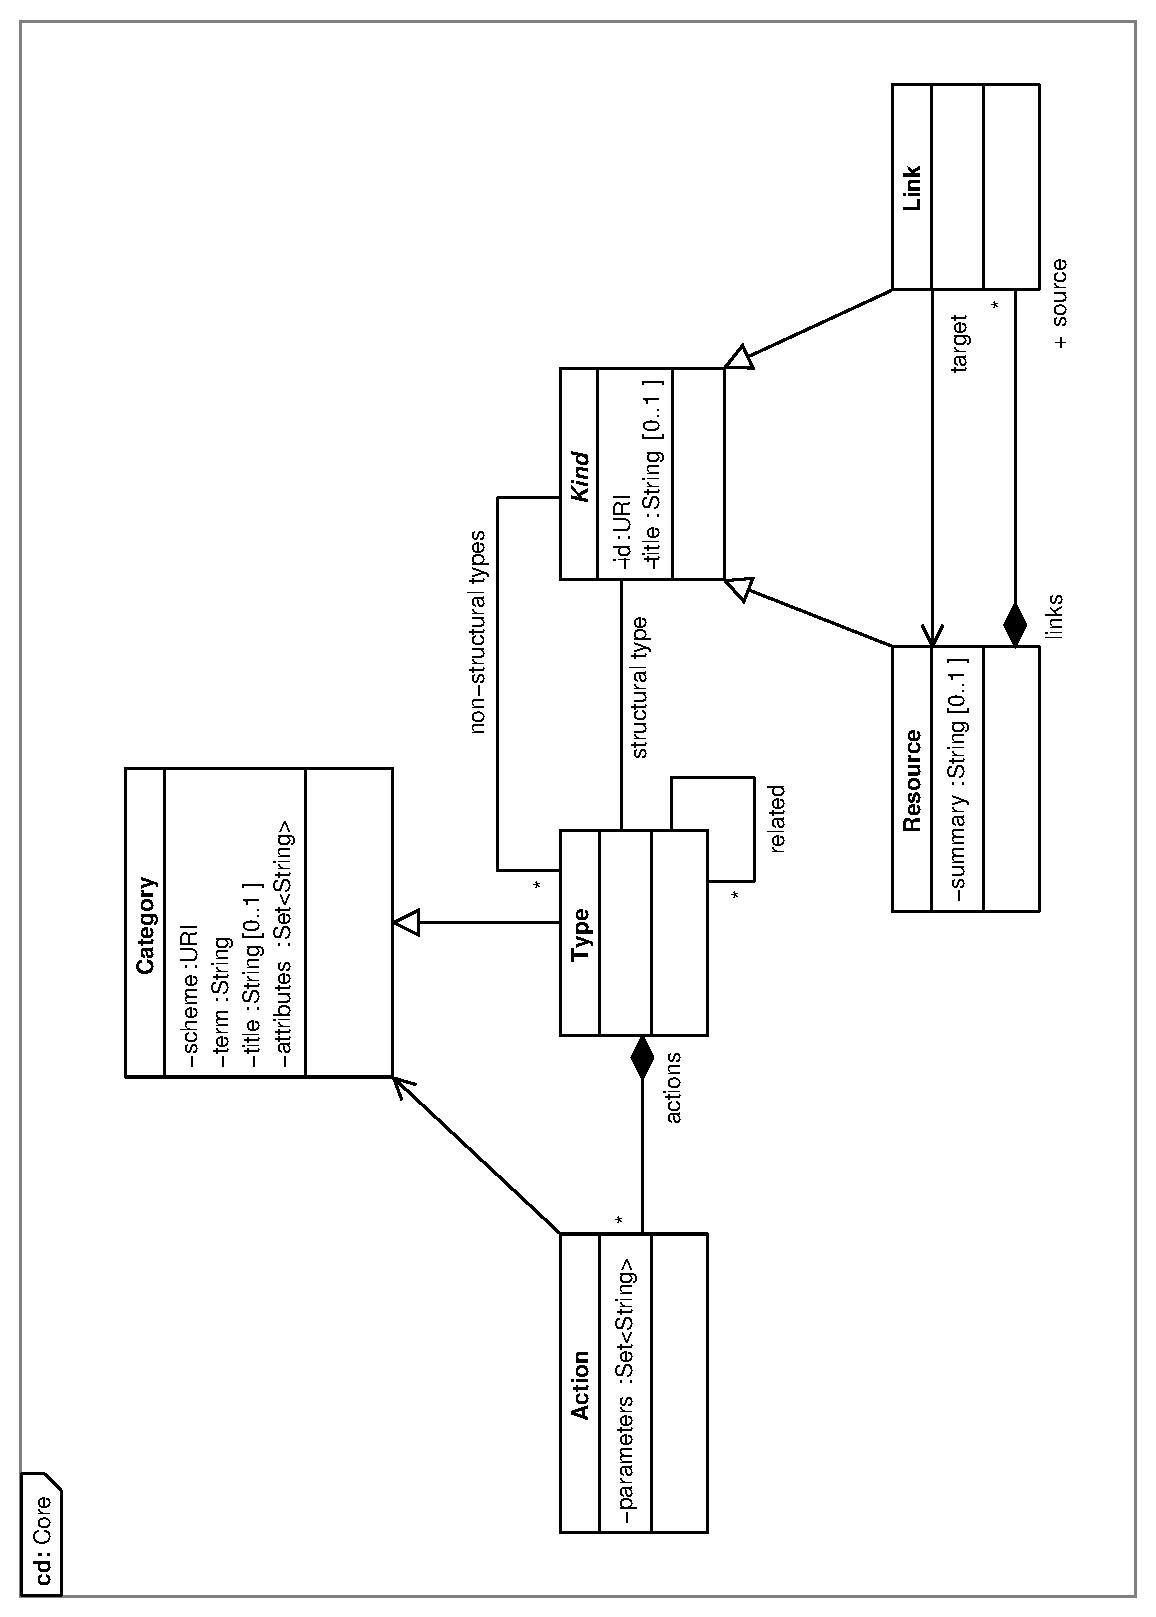
\includegraphics{figs/core_model.pdf}}} \par}
\caption{UML class diagram of the OCCI model. The diagram provides an
overview of the OCCI model but is not a standalone definition thereof}
\label{fig:occi_model}
\end{figure}

The UML class diagram shown in figure~\ref{fig:occi_model} gives an overview of
the OCCI model. It must be noted that the UML diagram in itself is not a
complete definition of the model. The diagram is merely provided as an overview
to help understanding the model.  The following sections of the specification
contain the formal definition of the OCCI model.

\subsection{Terms and definitions}
Section \ref{sec:glossary} provide a glossary of all terms and definitions with
a specific meaning to the OCCI specification suite. However, for reader
convenience, a sub-set of the glossary is provided here as well. The following
terminology have specific meaning in the OCCI context:
\begin{description}
\item[instance] An {\bf instance} refer to the instantiated object of a type
 defined in the OCCI model.
\item[mix-in] An instance of the \hl{Mixin} type associated with a {\bf resource
 instance}. The ``mix-in'' concept as used by OCCI {\em only} applies to
 instances, never to \hl{Entity} types.
\item[OCCI base type] The OCCI base types are \hl{Entity}, \hl{Resource},
 \hl{Link} and \hl{Action}.
\item[resource instance] An instance of a sub-type of \hl{Entity}. The OCCI
 model defines two sub-types of \hl{Entity}, the \hl{Resource} type and the
 \hl{Link} type.  However, the term {\bf resource instance} is defined to
 include any instance of a {\em sub-type} of \hl{Resource} or \hl{Link} as
 well.
\item[type] A {\bf type} refer to one of the types, i.e.~classes, defined by
 the OCCI model.
\end{description}

\subsection{Classification and Identification}
\label{sec:classification}
The OCCI model provides a built in classification system allowing for safe
extension towards domain-specific usage. This system is like a ``type system''
but with the possibility of being easily exposed over a text based protocol.
%
The classification system can be summarised with the following key features:
\begin{itemize}
\item Each OCCI base type and extension thereof is assigned a unique
 identifier, a \hl{Kind} instance, which allow for dynamic discovery of
 available types. All \hl{Entity} sub-types, including extensions, are assigned
 a unique \hl{Kind} instance.
\item The relationship of \hl{Kind} instances reflect the inheritance structure
 starting at \hl{Entity} type, the parent of all extensions. This makes it
 possible for an OCCI client to discover the inheritance structure of a
 particular OCCI implementation.
\item The classification system allows \hl{Mixin} instances to be associated
 to resource instances in order to assign additional capabilities in terms of
 attributes and \hl{Action}s at run-time.
\item Tagging of resource instances is supported through the association
 of \hl{Mixin} instances. A tag is simply a \hl{Mixin} instance which define no
 additional capabilities.
\item A collection of associated resource instances is implicitly defined for
 each \hl{Kind} and \hl{Mixin} instance. I.e.~all resource instances associated
 with a particular \hl{Kind} or \hl{Mixin} instance form a collection.
\end{itemize}

\subsubsection{Kind}
\label{sec:kind}
The \hl{Kind} type, together with the \hl{Mixin} type, define the
classification system of the OCCI model. It MUST be implemented. The \hl{Kind}
type represent the identification mechanism for all \hl{Entity} types present in
the model.

A \hl{Kind} {\em instance} is assigned to each and every \hl{Entity} sub-type
defined in an OCCI implementation. The capabilities, in terms of attributes and
\hl{Action}s, represented by a \hl{Kind} instance describe the capabilities of
its \hl{Entity} sub-type.
%
In a clean instantiation of the OCCI model, with no extensions, three instances
of \hl{Kind} will be present: one for \hl{Entity}, another for \hl{Resource}
and the last one for \hl{Link}. 

Every resource instance MUST be associated with the \hl{Kind} instance of its
\hl{Entity} sub-type. For example an instance of \hl{Resource} MUST be
associated with the \hl{Kind} instance which identify the \hl{Resource} {\em
type}.

\mytablefloat{\label{tbl:type}Attributes defined for the \hl{Kind} type}{
\begin{tabular}{llllp{2.7in}}
\toprule
Attribute & Type & Multiplicity & Client Mutability & Description \\
\colrule
actions & \hl{Action} & 0..* & Immutable & Set of \hl{Action}s defined by the \hl{Kind} instance. \\
related & \hl{Kind} & 0..* & Immutable & Set of related \hl{Kind} instances. \\
entity\_type & \hl{Entity} & 1 & Immutable & \hl{Entity} type uniquely identified by the \hl{Kind} instance. \\
entities & \hl{Entity} & 0..* & Immutable & Set of resource instances, i.e.~\hl{Entity} sub-type instances, uniquely identified by the \hl{Kind} instance. \\
\botrule
\end{tabular}
}
The \hl{Kind} type inherits the \hl{Category} type and all inherited
attributes MUST be implemented. Table~\ref{tbl:type} defines the
additional attributes the \hl{Kind} type MUST implement to be compliant.

A unique \hl{Kind} instance is assigned as the unique identifier of every
\hl{Entity} sub-type, including \hl{Entity} itself. The following rules apply
to the \hl{Kind} type:
\begin{itemize}
\item A unique \hl{Kind} instance MUST be assigned to each and every sub-type
 of \hl{Entity}.
\item A \hl{Kind} instance MUST define all capabilities of its \hl{Entity}
 sub-type in terms of attributes and \hl{Action}s. If an \hl{Entity} sub-type
 has an attribute named {\bf X}, the corresponding \hl{Kind} instance MUST define
 an attribute named {\bf X}.
\item A \hl{Kind} instance MUST be related, either directly or indirectly, to
 the \hl{Kind} instance of \hl{Entity},
 i.e. \textit{http://schemas.ogf.org/occi/core\#entity}.
 %
 See section~\ref{sec:type_relationship} for the definition of \hl{Kind}
 relationships.
\item If type {\bf B} inherit type {\bf A}, where {\bf A} is a sub-type of
 \hl{Entity}, the \hl{Kind} instance of {\bf B} MUST be directly related to the
 \hl{Kind} instance of {\bf A}.
\end{itemize}

\subsubsection{Mixin}
The \hl{Mixin} type complement the \hl{Kind} type in defining the
classification system of the OCCI model. It MUST be implemented. The \hl{Mixin}
type represent a run-time extension mechanism which allow new capabilities to
be added to existing resource instances.

A \hl{Mixin} {\em instance} can be associated with a resource instance and thereby
add the capabilities 

\mytablefloat{\label{tbl:type}Attributes defined for the \hl{Mixin} type}{
\begin{tabular}{llllp{2.7in}}
\toprule
Attribute & Type & Multiplicity & Client Mutability & Description \\
\colrule
actions & \hl{Action} & 0..* & Immutable & Set of \hl{Action}s defined by the \hl{Mixin} instance. \\
related & \hl{Mixin} & 0..* & Immutable & Set of related \hl{Mixin} instances. \\
entities & \hl{Entity} & 0..* & Immutable & Set of resource instances, i.e.~\hl{Entity} sub-type instances, associated with the \hl{Mixin} instance. \\
\botrule
\end{tabular}
}
The \hl{Mixin} type inherits the \hl{Category} type and all inherited
attributes MUST be implemented. Table~\ref{tbl:type} defines the
additional attributes the \hl{Mixin} type MUST implement to be compliant.

\paragraph*{Non-structural Kind} A non-structural \hl{Kind} is an instance of
\hl{Kind} {\em not} assigned as the unique identifier of any \hl{Entity} sub-type.
The following rules apply:
\begin{itemize}
\item A non-structural \hl{Kind} define additional capabilities for each
 \hl{Entity} sub-type instance it is associated with. A non-structural \hl{Kind}
 add capabilities using a mix-in like model.
\item A non-structural \hl{Kind} MUST only be associated with \hl{Entity}
 sub-type {\em instances}, either at creation-time or run-time.
\item A non-structural \hl{Kind} MUST NOT be related, neither directly nor
 indirectly, to the structural \hl{Kind} of \hl{Entity},
 i.e.~\textit{http://schemas.ogf.org/occi/core\#entity}.
 %
 See section~\ref{sec:type_relationship} for the definition of \hl{Kind}
 relationship.
\item A non-structural \hl{Kind} defining no additional capabilities in terms
 of attributes or \hl{Action}s is considered to be a tag.
\end{itemize}

\subsubsection{Category}
\label{sec:category}
The \hl{Category} type comprises the basis of the identification mechanism used
by the OCCI classification system. It MUST be implemented. Instances of the
\hl{Category} type are only used to identify \hl{Action} types. All other uses
of \hl{Category} properties are managed through its sub-type \hl{Kind}.
%
Table~\ref{tbl:category} defines the attributes the \hl{Category} type MUST
implement to be compliant.

\mytablefloat{\label{tbl:category}Attributes defined for the \hl{Category} type}{
\begin{tabular}{llllp{2.7in}}
\toprule
Attribute & Type & Multiplicity & Client Mutability & Description \\
\colrule
term & String & 1 & Immutable & Unique identifier of the \hl{Category} instance within the categorisation scheme. \\
scheme & URI & 1 & Immutable & The categorisation scheme. \\
title & String & 0..1 & Immutable & The display name of an instance. \\
attributes & String & 0..* & Immutable & The set of resource attribute names defined by the \hl{Category} instance. \\
\botrule
\end{tabular}
}

A \hl{Category} is uniquely identified by concatenating the categorisation
scheme with the category term,
e.g.~\textit{http://example.com/category/scheme\#term}.
This is done to enable discovery of \hl{Category} definitions in text based
renderings such as HTTP. All renderings MUST make use of and understand
concatenated unique identifiers of \hl{Category} types.
%
Sub-types of \hl{Category} such as \hl{Kind} inherit this property.

The categorisation schemes defined in the OCCI specification all use the
\textit{http://schemas.ogf.org/occi/} base URL. This base URL is reserved for
OCCI an MUST NOT be used by domain-specific extensions.

Attribute names defined by \hl{Category} instances%
\footnote{Also applies to \hl{Kind} instances.}
use the \texttt{occi.}~prefix.  This prefix is reserved for OCCI and MUST NOT
be used by domain-specific extensions.

\subsubsection{Kind relationship}
\label{sec:type_relationship}
As previously defined a structural \hl{Kind} MUST be related, either
either directly or indirectly, to the structural \hl{Kind} of \hl{Entity},
i.e.~\textit{http://schemas.ogf.org/occi/core\#entity}.
%
The OCCI base types \hl{Resource} and \hl{Link} extend \hl{Entity}.  This
together with any further sub-typing implies a hierarchy of related structural
\hl{Kind} instances.  The \hl{Kind} relationships thus mirror the type
inheritance structure of the OCCI model and any extension thereof.

In an example where a domain-specific ``Custom Compute Resource'' is a sub-type
the OCCI infrastructure type Compute, which in turn is a sub-type of the
\hl{Resource} type, four related structural \hl{Kind}s would be involved.
%
Table~\ref{tbl:relationship} illustrates the exemplified hierarchy of \hl{Kind}
instances relating the domain-specific structural \hl{Kind} to the structural
\hl{Kind} of \hl{Entity}.

\mytablefloat{\label{tbl:relationship}Example of the \hl{Kind} relationship involved
for a domain-specific extension of the OCCI infrastructure type \hl{Compute}.}{
\begin{tabular}{p{7cm}p{7cm}}
\toprule
Structural Kind & Related Structural Kind \\
\colrule
\textit{http://example.com/occi/custom\#compute} & \textit{http://schemas.ogf.org/occi/infrastructure\#compute} \\
\textit{http://schemas.ogf.org/occi/infrastructure\#compute} & \textit{http://schemas.ogf.org/occi/core\#resource} \\
\textit{http://schemas.ogf.org/occi/core\#resource} & \textit{http://schemas.ogf.org/occi/core\#entity} \\
\botrule
\end{tabular}
}

\subsubsection{Kind assignment}
\label{sec:type_assignment}
A structural \hl{Kind} MUST be statically assigned to each sub-type of
\hl{Entity} defined by an implementation. An \hl{Entity} sub-type instance MUST be
automatically associated with its structural \hl{Kind} at creation-time.  The
structural \hl{Kind} associated with an instance MUST remain associated with the
instance during its lifetime.

A non-structural \hl{Kind}, also known as a mix-in, MAY be associated with an
\hl{Entity} sub-type instance, either at creation-time or run-time. An OCCI
implementation MAY restrict which instances can be associated with a particular
non-structural \hl{Kind}.

\subsubsection{Collections}
\label{sec:collection}
One or more \hl{Entity} sub-type instances associated with the same \hl{Kind},
may it be structural or non-structural, automatically form a collection.
Each \hl{Kind} instance in the system identifies a collection consisting of all
different \hl{Entity} sub-type instances associated with the \hl{Kind}.

An \hl{Entity} sub-type instance is always a member of the collection implied
by the \hl{Entity}'s structural \hl{Kind}. This follows from the rule that an
\hl{Entity} sub-type instance MUST be associated with the structural \hl{Kind}
assigned to the sub-type.
Since a non-structural \hl{Kind} can be assigned to any \hl{Entity} sub-type
instance a collection can contain instances of different \hl{Entity} sub-types.
%
For example, an instance of the \hl{Resource} type will always be associated
to the structural \hl{Kind}
\textit{http://scheme.ogf.org/occi/core\#resource} and thus part of the
collection implied by the \hl{Kind}.
\begin{description}
\item[Adding an instance] to a collection is accomplished by associating the
corresponding non-structural \hl{Kind} to the \hl{Entity} sub-type instance.
\item[Removing an instance] from a collection is accomplished by disassociating the
corresponding non-structural \hl{Kind} from the \hl{Entity} sub-type instance.
\end{description}
%
An OCCI implementation MUST allow a client to navigate collections. The
following basic navigation operations MUST be supported:
\begin{itemize}
\item Retrieve the whole collection.
\item Retrieve a specific item in a collection.
\item Retrieve a subset of a collection.
\end{itemize}
The details of collection navigation is rendering specific.

\subsubsection{Discovery}
\label{sec:discovery}
An OCCI client MUST be able to discover all instances of \hl{Kind} and
\hl{Category} a particular service provider's OCCI implementation support. By
examining these instances a client MUST be able to, at a minimum, deduce the
following information:
\begin{itemize}
\item The \hl{Entity} sub-types available from a the service provider, including domain-specific extensions.
\item The attributes associated with each \hl{Entity} sub-type.
\item The invocable operations, i.e. \hl{Action}s, defined for each \hl{Entity} sub-type.
\item Additional mix-ins or tags, i.e. non-structural \hl{Kind}s, applicable to
 \hl{Entity} sub-type instances.
\end{itemize}
The above requirements comprise the OCCI discovery mechanism. It MUST be
implemented.
%
The details of exactly how the \hl{Category} and \hl{Kind} instances are
exposed to an OCCI client is specific to the particular rendering used.
\marginpar{References?}
The relevant details can be found in the OCCI rendering documents.

%%%%%%%%%%%%%%%%%%%%%%%%%%%%% Bits and pieces %%%%%%%%%%%%%%%%%%%%%%%%%%%%%%%%%%

% Stuff which may or may not be useful to add somewhere in the spec...

\begin{comment}
The central component of the classification system is the \hl{Kind} type which
is a specialisation of the \hl{Category} type. The following sections describe
the OCCI classification system in detail.

Each OCCI base type, see section~\ref{sec:base_types}, is assigned a
unique identifier.  This identifier is an instance of \hl{Kind} and comprise
the structural \hl{Kind} of the associated base type%
\footnote{The \hl{Action} type is an exception and is instead uniquely
identified by a \hl{Category} instance. An \hl{Action} is a capability of \hl{Kind}
and can therefore not be identified by \hl{Kind}.}.
\end{comment}


\begin{comment}
%%% CLIENT Interaction, do we need to specify this explicitly?!
\subsubsection{Creating Instances}
A client MUST supply the concrete Entity type as a Category. All OCCI
implementations MUST understand these requests containing concrete
Entity types, i.e. Resource, Link, Action or a subtype thereof.

When a client attempts to add a non-structural
\hl{Kind} at a stage not supported by a particular provider's OCCI
implementation, the provider MUST notify the client it has issued a bad
request.
\end{comment}

%%%%%%%%%%%%%%%%%%%%%%%%%%%%%%%%%%%%%%%%%%%%%%%%%%%%%%%%%%%%%%%%%%%%%%%%%%%%%%%


\subsection{The OCCI base types}
\label{sec:base_types}
The following sections describe the OCCI base types defined by the OCCI model.
The base types are \hl{Entity}, \hl{Resource}, \hl{Link} and \hl{Action}. All
base types MUST be implemented.

\subsubsection{Entity}
\label{sec:entity}
The \hl{Entity} type is the abstract base type for \hl{Resource} and \hl{Link}
and any domain-specific sub-types thereof. It MUST be implemented.
%
Table~\ref{tbl:entity} defines the attributes the \hl{Entity} type MUST implement to
be compliant.

\mytablefloat{\label{tbl:entity}Attributes defined for the \hl{Entity} type.}{
\begin{tabular}{llllp{7cm}}
\toprule
Attribute & Type & Multiplicity & Client Mutability & Description \\
\colrule
id & URI & 1 & Immutable & A unique identifier (within the service provider's name-space) of the \hl{Entity} sub-type instance. \\
title & String & 0..1 & Mutable & The display name of the instance. \\
structural kind & \hl{Kind} & 1 & Immutable & The structural \hl{Kind} of the instance. \\
non-structural kinds & \hl{Kind} & 0..* & Mutable & The non-structural \hl{Kind}s associated to this instance. Consumers can expect the attributes and \hl{Action}s of the associated non-structural \hl{Kind}s to be exposed by the instance. \\ 
\botrule
\end{tabular}
}

\hl{Entity} enforces for all sub-types a required \texttt{id} attribute and an
optional \texttt{title} attribute.
%
Every sub-type of \hl{Entity} MUST be assigned a structural \hl{Kind}, see
section~\ref{sec:type}. \hl{Entity} itself is assigned the structural \hl{Kind}
\textit{http://schemas.ogf.org/occi/core\#entity}.
%
An \hl{Entity} sub-type instance MAY be associated with one or more non-structural
\hl{Kind}s.

An \hl{Entity} sub-type instance MUST expose its structural \hl{Kind} and any
associated non-structural \hl{Kind}s together with their associated attributes
and \hl{Action}s.

\subsubsection{Resource}
\label{sec:resource}
The \hl{Resource} type inherit \hl{Entity} and describes a concrete resource that
can be inspected and manipulated. It represents a general object in the OCCI
model and MUST be implemented.
%
The \hl{Resource} type MUST implement all attributes inherited from the
\hl{Entity} type together with the attributes defined in table~\ref{tbl:resource}
in order to be compliant.
%
The Resource type is assigned the structural \hl{Kind}
\textit{http://schemas.ogf.org/occi/core\#resource}.

\mytablefloat{\label{tbl:resource}Attributes defined for the \hl{Resource} type.}{
\begin{tabular}{llllp{8cm}}
\toprule
Attribute & Type & Multiplicity & Client Mutability & Description \\
\colrule
summary & String & 0..1 & Mutable & A summarising description of the \hl{Resource} instance.\\
links & \hl{Link} & 0..* & Mutable & A set of \hl{Link} compositions. Being a composite relation the removal of a \hl{Link} from the set MUST also remove the \hl{Link} instance.\\
\botrule
\end{tabular}
}

\hl{Resource} enforces the inheritance of a set of common attributes into
sub-types. Moreover, it introduces relationships to other \hl{Resource}
instances through instances of the \hl{Link} type.
%
The \hl{Resource} type is the entry point for domain-specific extensions of the
OCCI model, see section~\ref{sec:extensibility}.

\subsubsection{Link}
\label{sec:link}
An instance of the \hl{Link} type defines a base association between two
\hl{Resource} instances. It MUST be implemented. A \hl{Link} instance indicates
that one \hl{Resource} instance is connected to another.
%
The \hl{Link} type MUST implement all attributes inherited from the
\hl{Entity} type together with the attributes defined in table~\ref{tbl:link}
in order to be compliant.
%
The Link type is assigned the structural \hl{Kind}
\textit{http://schemas.ogf.org/occi/core\#link}.

\mytablefloat{\label{tbl:link}Attributes defined for the \hl{Link} type.}{
\begin{tabular}{llllp{7.5cm}}
\toprule
Attribute & Type & Multiplicity & Client Mutability & Description \\
\colrule
source & \hl{Resource} & 1 & Mutable & The \hl{Resource} instances the \hl{Link} instance originates from.\\
target & \hl{Resource} & 1 & Mutable & The \hl{Resource} instances the \hl{Link} instance points to.\\
\botrule
\end{tabular}
}

An instance of the \hl{Link} type MUST NOT refer to an external resource.  A
provider MAY however create a sub-type of \hl{Link} with different semantics,
e.g.~have a target attribute containing an URI and thus the ability of linking
with external resources.
%
The \hl{Link} type can be sub-typed for domain-specific extensions of the
OCCI model, see section~\ref{sec:extensibility}.

\subsubsection{Action}
The \hl{Action} type defines an invocable operation applicable to an \hl{Entity}
sub-type instance or a collection thereof. It MUST be implemented. In general,
\hl{Action}s modify state by e.g.~performing a complex operation such as
rebooting a virtual machine.
%
Table~\ref{tbl:action} defines the attributes the \hl{Action} type MUST
implement to be compliant.

\mytablefloat{\label{tbl:action}Attributes defined for the \hl{Action} type.}{
\begin{tabular}{llllp{7.5cm}}
\toprule
Attribute & Type & Multiplicity & Client Mutability & Description \\
\colrule
category & \hl{Category} & 1 & Immutable & The identifying \hl{Category} of the \hl{Action}. \\
parameters & String & 0..* & Immutable & Enumeration of valid parameters for the \hl{Action}. \\
\botrule
\end{tabular}
}

An \hl{Action} is always bound to a \hl{Kind} instance through a composite
association. An \hl{Action} is considered a capability of the \hl{Kind}.  An
\hl{Action} MAY be invoked on any \hl{Entity} sub-type instance associated with
the \hl{Kind} instance defining the \hl{Action}. An OCCI implementation MAY
refuse an \hl{Action} from being invoked if currently not applicable.

An \hl{Action} MAY be invoked on a collection of \hl{Entity} sub-type instances.
The \hl{Action} is only considered valid if all instances of the collection are
associated with the \hl{Kind} defining the \hl{Action}.

The Action type is assigned the \hl{Category} identifier
\textit{http://schemas.ogf.org/occi/core\#action}.
%
The \hl{Action} type can be sub-typed for domain-specific extensions of the
OCCI model, see section~\ref{sec:extensibility}.

\subsection{Mutability}
Attributes of an OCCI model type instance, a resource instance, are
either client mutable or client immutable. If an attribute is noted to
be mutable this MUST be interpreted that a client can create a
resource instance that is parametrised by the attribute. Likewise, if
an attribute is mutable, a client can update that resource instance's
mutable attribute value and the server side MUST support this. If an
attribute is marked as immutable, it indicates that the server side
implementation MUST manage these exclusively. Immutable attributes
MUST NOT be modifiable by clients under any circumstance.

\subsection{Extensibility}
\label{sec:extensibility}
The OCCI model has a flexible yet fairly simple extension mechanism based on
the classification system described in section~\ref{sec:classification}.
%
The OCCI model can be extended using two different methods, sub-typing and
mix-in. Custom sub-typing require domain-specific \hl{Kind} instances and
custom mix-ins require domain-specific \hl{Mixin} instances.  Both methods MAY
involve the use of domain-specific \hl{Category} instance since those are
REQUIRED for domain-specific \hl{Action} sub-types.  The following sections
define the rules for extensions of the OCCI model.
%
The rules defined in section~\ref{sec:classification} and \ref{sec:base_types}
are REQUIRED for all extensions of the OCCI model.

\subsubsection{\hl{Category} instances}
\label{sec:ext:category}
Domain-specific instances of \hl{Category}, \hl{Kind} and \hl{Mixin} MAY be
introduced by an OCCI implementation. Since \hl{Kind} and \hl{Mixin} both
inherit \hl{Category} the extension rules for \hl{Category}, defined below,
applies to them as well.

A \hl{Category} instance defined outside of the OCCI specification MUST use a
categorisation scheme unique to the provider,
e.g.~\textit{http://example.com/occi\#}.
%
An attribute introduced by a domain-specific \hl{Category} MUST
use an attribute name prefix. This prefix MUST NOT be the ``\texttt{occi.}''~prefix
which is reserved for the OCCI specification. Domain-specific attribute names
SHOULD use a prefix consisting of the provider's reverse domain name,
e.g.~``\texttt{com.example.}''.

\subsubsection{Sub-typing}
The OCCI model MAY be extended through sub-typing for domain-specific purposes.
Three OCCI model types MAY be sub-typed, those are \hl{Resource}, \hl{Link} and
\hl{Action}.

In order to define a sub-type of \hl{Resource} or \hl{Link} a domain-specific
\hl{Kind} instance MUST be defined and assigned to the sub-type. This
\hl{Kind} instance MUST be directly related to the \hl{Kind} instance of the
type extended.

In order to define a sub-type of \hl{Action} a domain-specific \hl{Category}
instance MUST be assigned to the \hl{Action} sub-type as its unique identifier.
Furthermore the \hl{Action} sub-type MUST be associated as a capability of a
domain-specific \hl{Kind} or \hl{Mixin} instance.

\subsubsection{Mix-ins}
The OCCI model MAY be extended using a ``mix-in'' like model by defining
domain-specific \hl{Mixin} instances.  A \hl{Mixin} instance can be associated
with any resource instance although a provider MAY apply restrictions.

In order to support user-defined tags an OCCI implementation must allow custom
\hl{Mixin} instances to be created and destroyed by request of a client.
There is no limitation in the OCCI model from doing so but it is RECOMMENDED to
assign a separate categorisation scheme for each user's \hl{Mixin}%
\footnote{A tag is a \hl{Mixin} instance which does not introduce additional
capabilities.}
instances.

\section{Contributors}
Editors: Andy Edmonds, Thijs Metsch, Ralf Nyrén \\
Contributors: Alexander Papaspyrou, Sam Johnston

\textbf{TBD: Bunch op people missing here - create table\ldots}

\section{Glossary}
\label{sec:glossary}
\begin{tabular}{l|p{12cm}}
Term & Description \\
\hline
\hl{Action} & An OCCI base type. Represent an invocable operation on a \hl{Entity} sub-type instance or collection thereof. \\

\hl{Category} & A type in the OCCI model. The parent type of \hl{Kind}. \\

\hl{Client} & An OCCI client.\\

\hl{Collection} & A set of \hl{Entity} sub-type instances all associated to a particular \hl{Kind} or \hl{Mixin} instance. \\

\hl{Entity} & An OCCI base type. The parent type of \hl{Resource} and \hl{Link}. \\

\hl{Kind} & A type in the OCCI model. A core component of the OCCI classification system. \\

\hl{Link} & An OCCI base type. A \hl{Link} instance associate one \hl{Resource} instance with another. \\

mixin & An instance of the \hl{Mixin} type associated with a {\bf resource
 instance}. The ``mixin'' concept as used by OCCI {\em only} applies to
 instances, never to \hl{Entity} types. \\

\hl{Mixin} & A type in the OCCI model. A core component of the OCCI classification system. \\

\hl{OCCI} & Open Cloud Computing Interface \\

OCCI base type & One of \hl{Entity}, \hl{Resource}, \hl{Link} or \hl{Action}. \\

OGF & Open Grid Forum \\

\hl{Resource} & An OCCI base type. The parent type for all domain-specific resource types. \\

resource instance & An instance of a sub-type of \hl{Entity}. The OCCI
 model defines two sub-types of \hl{Entity}, the \hl{Resource} type and the
 \hl{Link} type. However, the term {\em resource instance} is defined to
 include any instance of a {\em sub-type} of \hl{Resource} or \hl{Link} as
 well. \\

Tag & A \hl{Mixin} instance with no attributes or actions defined. \\

Template & A \hl{Mixin} instance which if associated at resource instantiation
time pre-populate certain attributes. \\

type & One of the types defined by the OCCI model.  The OCCI model types are
 \hl{Category}, \hl{Kind}, \hl{Mixin}, \hl{Action}, \hl{Entity}, \hl{Resource}
 and \hl{Link}. \\

URI & Uniform Resource Identifier \\
URL & Uniform Resource Locator \\
URN & Uniform Resource Name \\
\end{tabular}



\section{Intellectual Property Statement}
The OGF takes no position regarding the validity or scope of any
intellectual property or other rights that might be claimed to pertain
to the implementation or use of the technology described in this
document or the extent to which any license under such rights might or
might not be available; neither does it represent that it has made any
effort to identify any such rights. Copies of claims of rights made
available for publication and any assurances of licenses to be made
available, or the result of an attempt made to obtain a general
license or permission for the use of such proprietary rights by
implementers or users of this specification can be obtained from the
OGF Secretariat.

The OGF invites any interested party to bring to its attention any
copyrights, patents or patent applications, or other proprietary
rights which may cover technology that may be required to practice
this recommendation. Please address the information to the OGF
Executive Director.


\section{Disclaimer}
This document and the information contained herein is provided on an
``As Is'' basis and the OGF disclaims all warranties, express or
implied, including but not limited to any warranty that the use of the
information herein will not infringe any rights or any implied
warranties of merchantability or fitness for a particular purpose.


\section{Full Copyright Notice}
Copyright \copyright ~Open Grid Forum (2009-2014). All Rights Reserved.

This document and translations of it may be copied and furnished to
others, and derivative works that comment on or otherwise explain it
or assist in its implementation may be prepared, copied, published and
distributed, in whole or in part, without restriction of any kind,
provided that the above copyright notice and this paragraph are
included on all such copies and derivative works. However, this
document itself may not be modified in any way, such as by removing
the copyright notice or references to the OGF or other organizations,
except as needed for the purpose of developing Grid Recommendations in
which case the procedures for copyrights defined in the OGF Document
process must be followed, or as required to translate it into
languages other than English.

The limited permissions granted above are perpetual and will not be
revoked by the OGF or its successors or assignees.


\section{References}

Note that only permanent documents should be cited as
references. Other items, such as Web pages or working groups, should
be cited inline (i.e., see the Open Grid Forum,
http://www.ogf.org). References should conform to a standard such as
used by IEEE/ACM, MLA, Chicago or similar. Include an author, year,
title, publisher, place of publication. For online materials, also add
a URL. It is acceptable to separate out ''normative references,'' as
IETF documents typically do. Some sample citations:

\end{document}
